\section{Result and discussion}
The YOLO-NAS has YOLO-NAS-L, YOLO-NAS-M, and YOLO-NAS-S variants, and in the result and discussion I am tailored to discuss individual performance characteristics of each model, and every model has three paths to choose from; the best model, average model, and latest model, and particularly I performed inference using the best weight of each model.

\subsection{Training and Implementation Details}
A batch size of 16 was used for all models, and they were trained for 60 epochs on NVIDIA Tesla T4 GPU with High-RAM. Before commencing training, various hyperparameters were adjusted. The "average best models" option was enabled, and warm-up models were set up with a linear epoch step. The initial learning rate was set to 1e-6 during warm-up, and the learning rate decay factor was set to 3. The initial learning rate was set to 5e-4, and the learning rate decay mode was cosine. The cosine-final learning rate ratio was set to 0.1, and the optimizer was Adam. The weight decay in optimizer parameters was set to 0.0001, and no weight decay was applied to bias and batch-normalization.
Furthermore, exponential moving averaging was used with a decay factor of 0.9, and the decay type was set to a threshold. The "mixed precision" option was enabled during training. All models were implemented and trained on Google Colab.
\subsubsection{YOLO-NAS-S}
The performance evaluation of inference on both models(i.e., before training and after training) is conducted utilizing a metric known as Intersection over Union (IoU) with a value of 0.5 and above and a confidence level of 0.5 and above. The images used to evaluate the model's performance are foreign images.
\begin{figure}[H]
  \centering
  \begin{subfigure}{\textwidth}
    \centering
    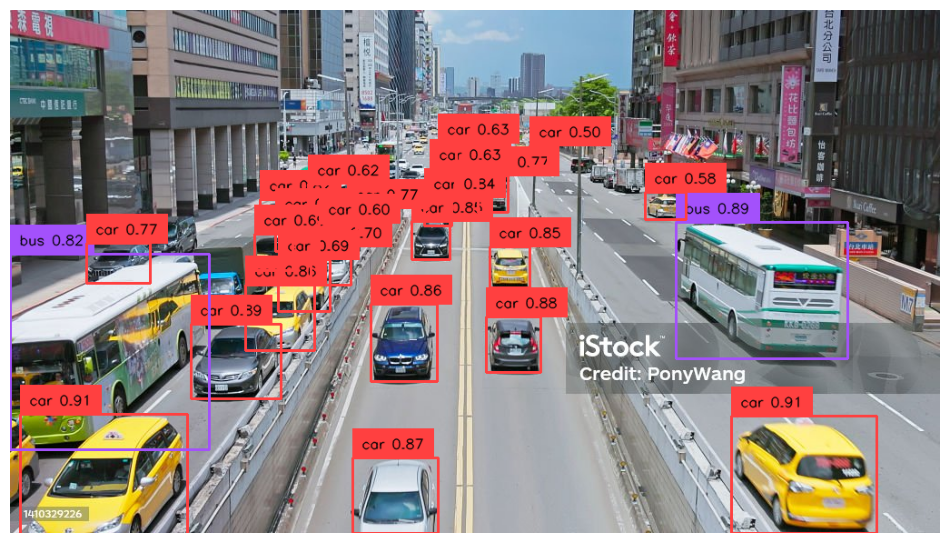
\includegraphics[width=\textwidth]{tex/img/YNS2_BT_3.png}
    \caption{YOLO-NAS-S: Inference on the Model before training}
    \label{fig:sub_s1}
  \end{subfigure}
  \hfill
  \begin{subfigure}{\textwidth}
    \centering
    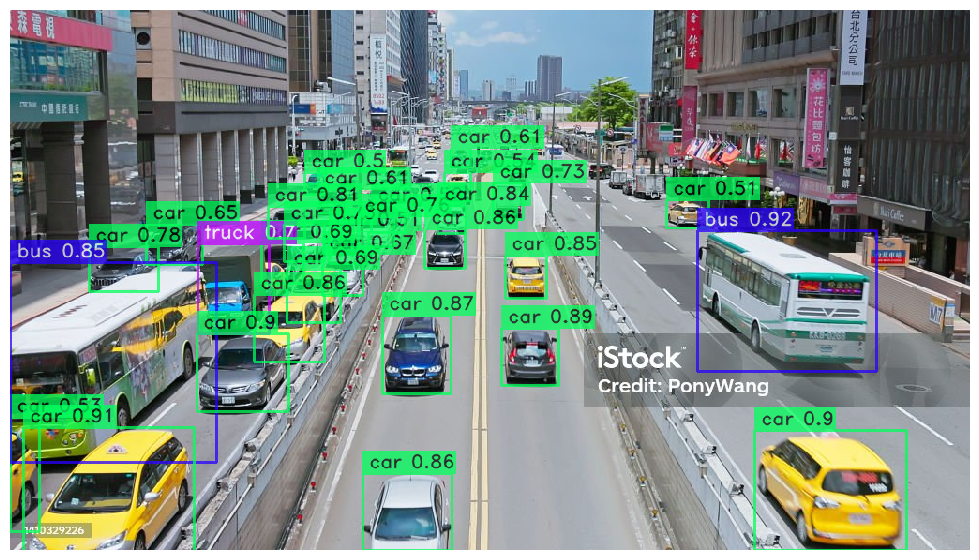
\includegraphics[width=\textwidth]{tex/img/YNS2_AT_3.png}
    \caption{YOLO-NAS-S: Inference on the Model after training}
    \label{fig:sub_s2}
  \end{subfigure}
  \caption{YOLO-NAS: Inference on the model before and  after training .}
  \label{fig:NAS-S} 
\end{figure}

Both models exhibit almost the same level of performance, but as can be seen from both images, the trained model outperforms with a slight difference where it shows a slightly better trade-off between precision and recall, also the dataset used for training is annotated mostly for not distant or short range, as a consequence the model is also exhibiting that it is struggling to detect the distant classes, sometimes the fine-tuned model is good at detecting distant objects.


 \begin{figure}[H]
    \centering
    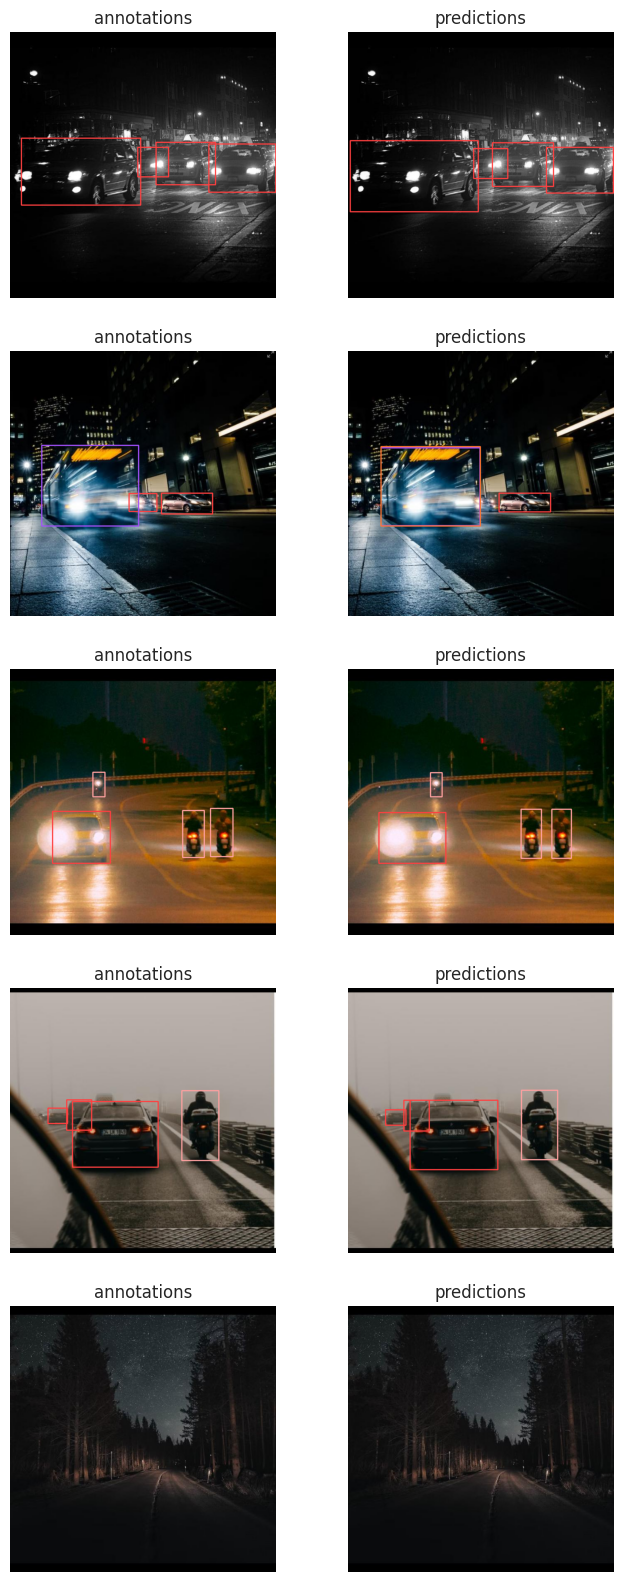
\includegraphics[width=0.5\linewidth]{tex/img/YNS2_AP_3.png}
    \caption{Visualization of the performance of YOLO-NAS-S with bounding boxes and corresponding obstacle
classes predicted by the model.}
    \label{fig:S-annot-pred}
\end{figure}

\begin{figure}[H]
The Confusion Matrix illustrates the effectiveness of the overall YOLO-NAS-S in detecting obstacles across four distinct classes. Notably, the matrix reveals a notable variation in the true positive values. Specifically, the highest true positive rate, standing at 1 which is not good, is achieved in detecting the 'motorbike' class. Conversely, the 'truck' class exhibits the lowest true positive rate, measured at 0.55.
    \centering
    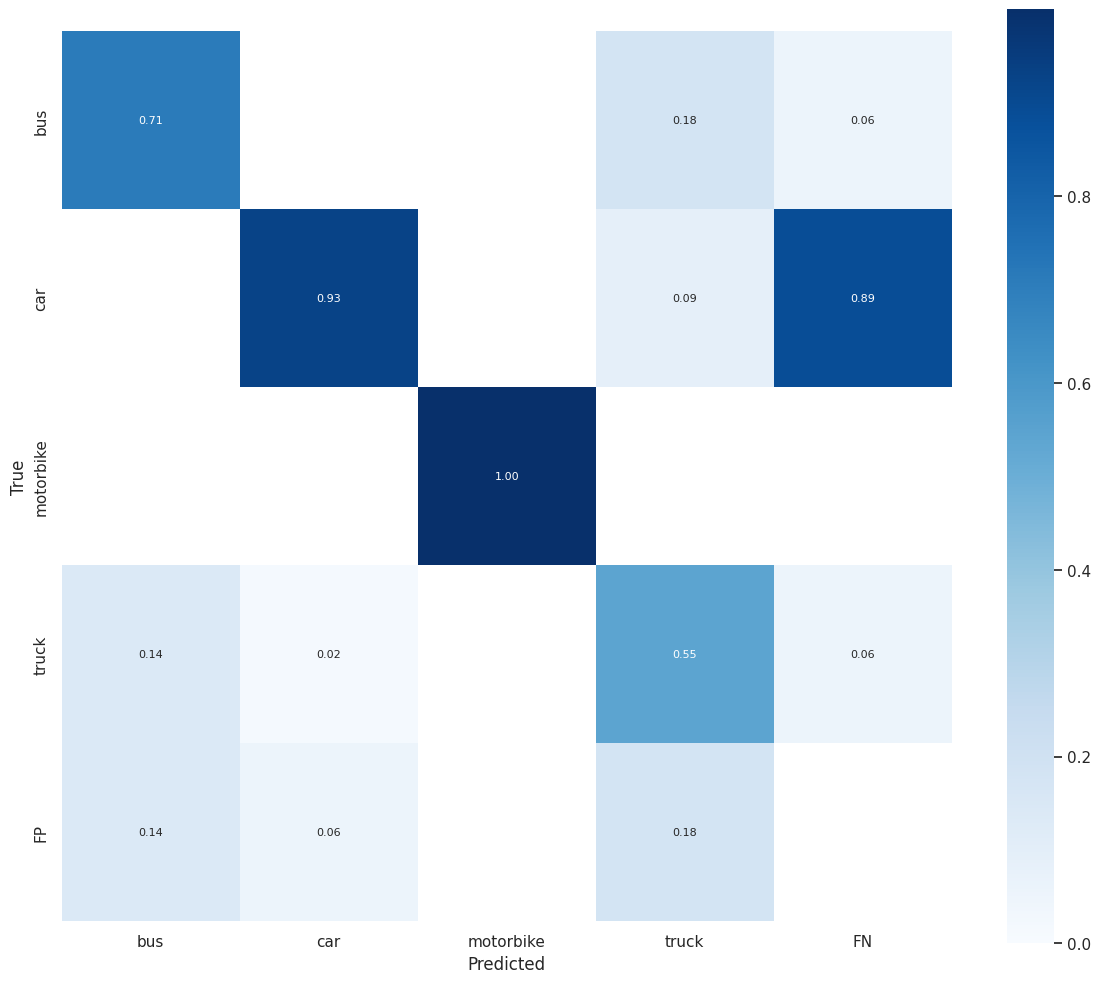
\includegraphics[width=\linewidth]{tex/img/YNS2_CM.png}
    \caption{YOLO-NAS-S Overall results }
    \label{fig:ConfusionMatrixY-N-S}
\end{figure}
%%%%%%%%%%%%%%%%%%%%%%%%
%YOLONAS-M
%%%%%%%%%%%%%%%%%%%%
\newpage
\subsubsection{YOLO-NAS-M}
The performance evaluation of inference for models is the same for all. As shown in \ref{fig:sub_M1}, The pre-trained model produces false positives, and after extensive training, the trained model exhibits very good results in detecting the short-range objects as YOLO-NAS-S model because of the dataset properties.
\begin{figure}[hpbt]
  \centering
  \begin{subfigure}{\textwidth}
    \centering
    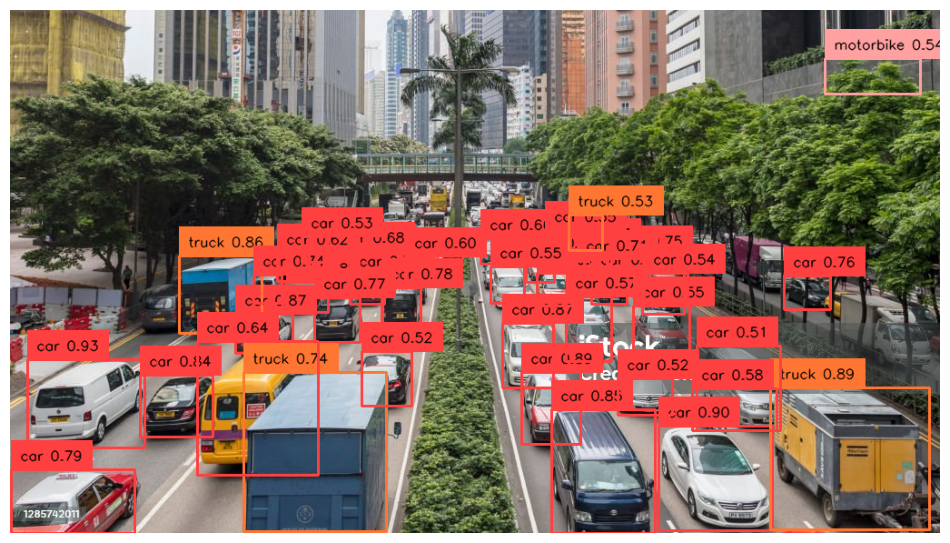
\includegraphics[width=0.9\textwidth]{tex/img/YNM2_BT_6.png}
    \caption{YOLO-NAS-M: Inference on the Model before training}
    \label{fig:sub_M1}
  \end{subfigure}
  \hfill
  \begin{subfigure}{\textwidth}
    \centering
    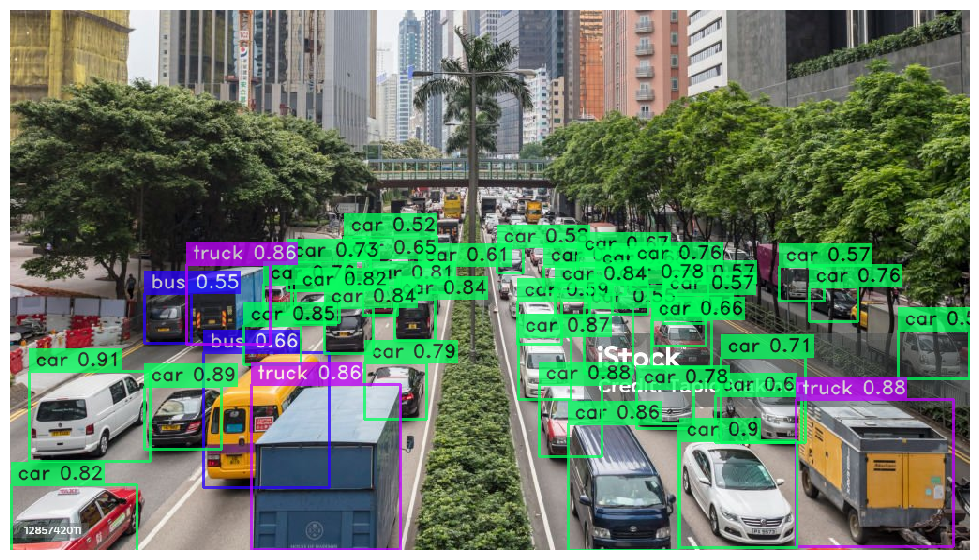
\includegraphics[width=0.9\textwidth]{tex/img/YNM2_AT_6.png}
    \caption{YOLO-NAS-M: Inference on the Model after training}
    \label{fig:sub_M2}
  \end{subfigure}
  \caption{YOLO-NAS-M: Inference on the model before and  after training .}
  \label{fig:NAS-M} 
\end{figure}



\begin{figure}[H]
    \centering
    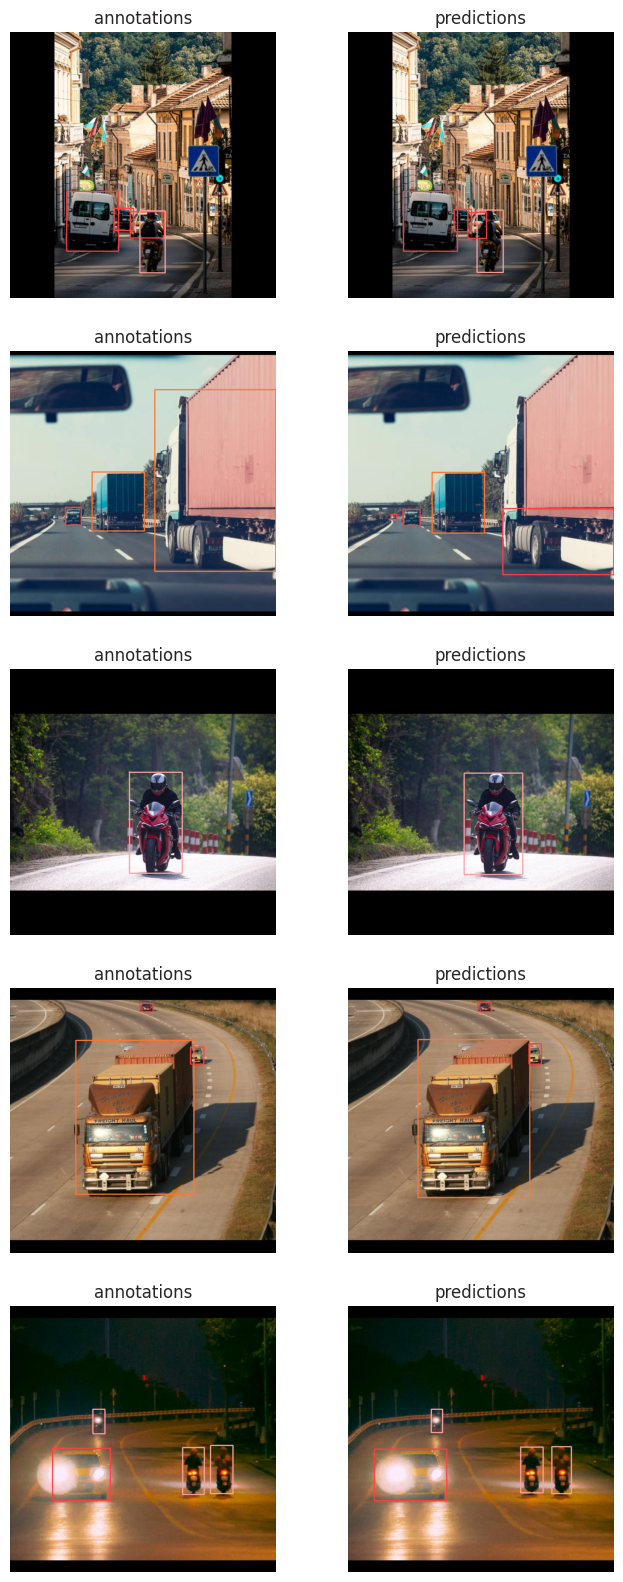
\includegraphics[width=0.6\linewidth]{tex/img/YNM2_AP_4.png}
    \caption{Visualization of the performance of YOLO-NAS-M with bounding boxes and corresponding obstacle
classes predicted by the model.}
    \label{fig:M-annot-pred}
\end{figure}

\begin{figure}[H]
The Confusion Matrix illustrates the effectiveness of the overall YOLO-NAS-M in detecting obstacles across four distinct classes. Notably, the matrix reveals a notable variation in the true positive values. Specifically, the highest true positive rate, standing at 0.93 which is good, is achieved in detecting the 'motorbike' class. Conversely, the 'truck' class exhibits the lowest true positive rate, measured at 0.56 which is better than the small model, from this we can tell that it is slightly better at balancing the trade-off between recall and precision, this is due to the size of the dataset in the backbone of the pre-trained model. The table shows that the model is losing to detect a car class or generates a significant number of false negatives for this category. This is likely attributed to the model's struggle in detecting distant cars.
    \centering
    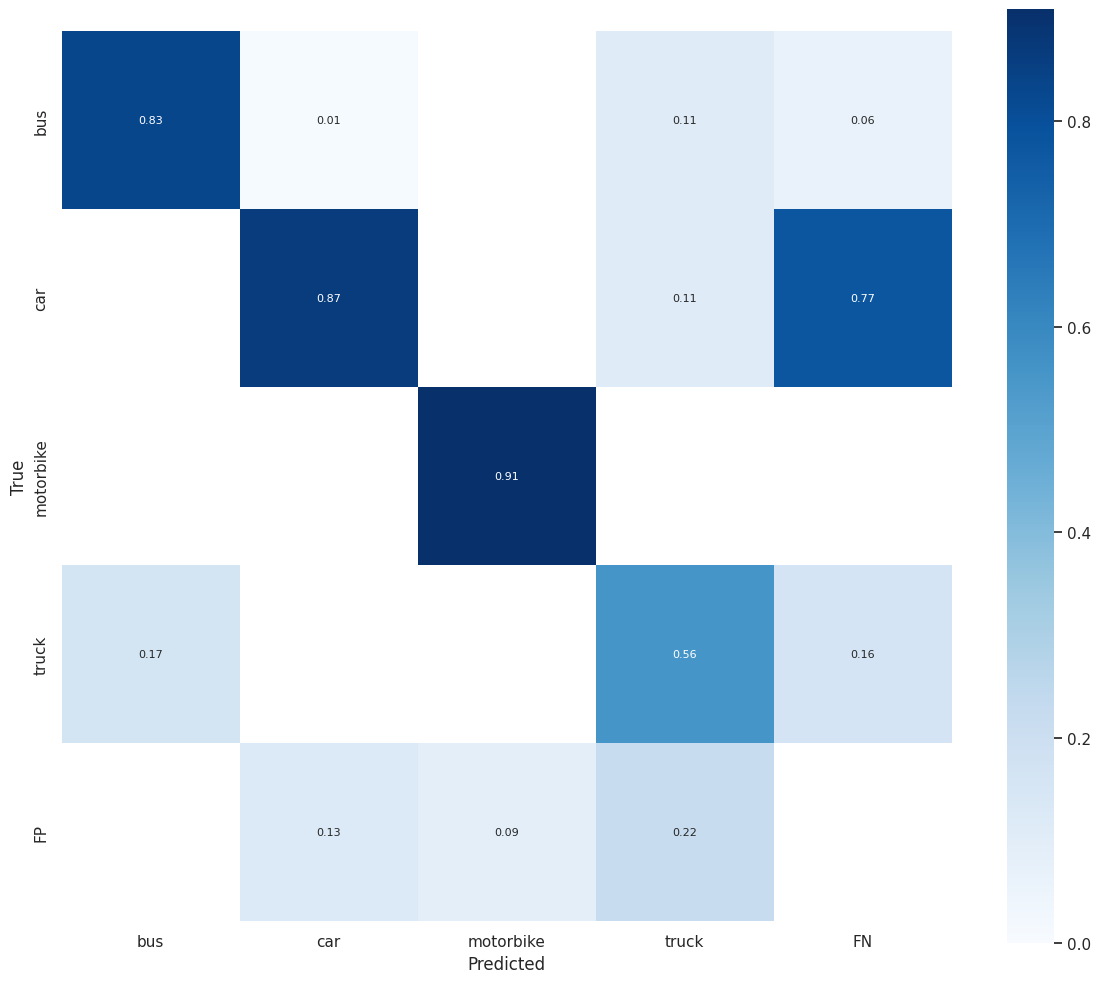
\includegraphics[width=\linewidth]{tex/img/YNM2_CM.png}
    \caption{YOLO-NAS-M Overall results }
    \label{fig:ConfusionMatrixY-N-M}
\end{figure}

%%%%%%%%%%%%%%%%%%%%%%%%%%%%%%
%YOLO-NAS-L
%%%%%%%%%%%%%%%%%%%%%%%%%%
\subsubsection{YOLO-NAS-L}
The performance evaluation of inference for models is the same for all.
As the model size of the pre-trained model increases, the model exhibits an increase in the trade-off between precision and recall and I will discuss extensively in Table: \ref{tab:my_label} 
\begin{figure}[H]
  \centering
  \begin{subfigure}{\textwidth}
    \centering
    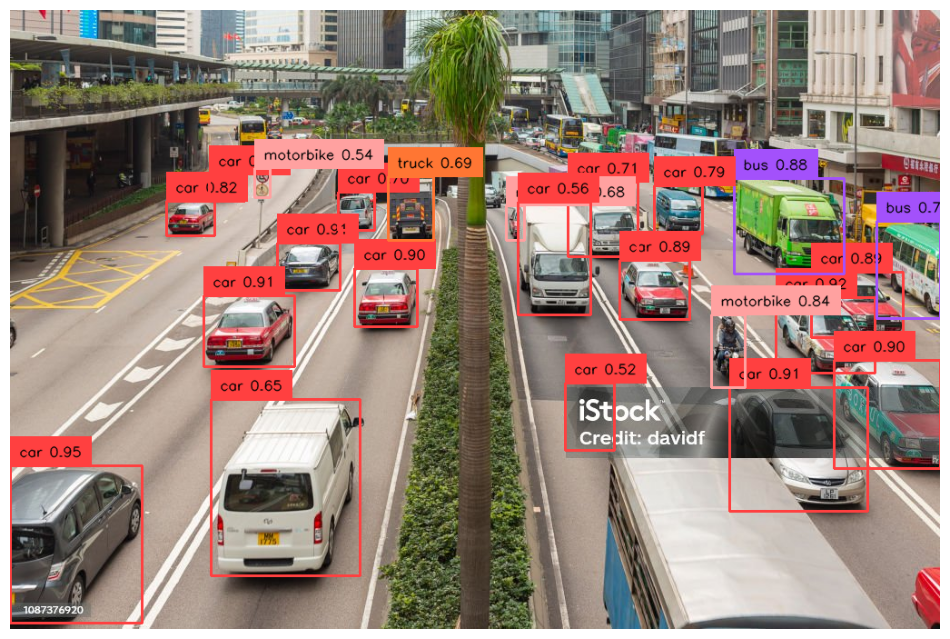
\includegraphics[width=\textwidth]{tex/img/YNL2__BT_6.png}
    \caption{YOLO-NAS-L: Inference on the Model before training}
    \label{fig:sub_M1}
  \end{subfigure}
  \hfill
  \begin{subfigure}{\textwidth}
    \centering
    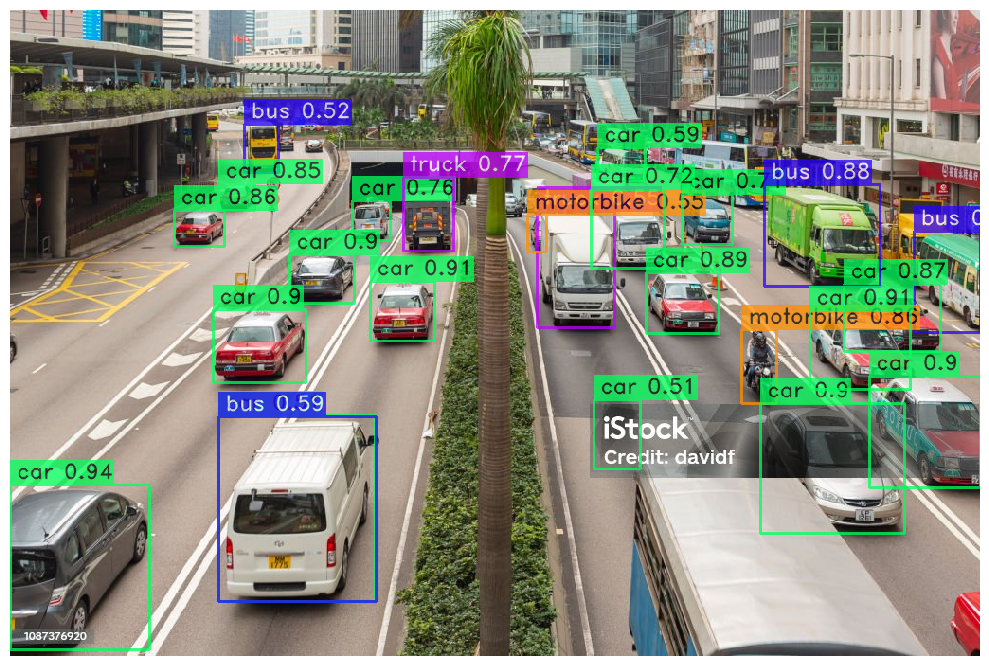
\includegraphics[width=\textwidth]{tex/img/YNL2__AT_6.png}
    \caption{YOLO-NAS-L: Inference on the Model after training}
    \label{fig:sub_M2}
  \end{subfigure}
  \caption{YOLO-NAS-L: Inference on the model before and  after training .}
  \label{fig:NAS-L} 
\end{figure}


\begin{figure}[H]
    \centering
    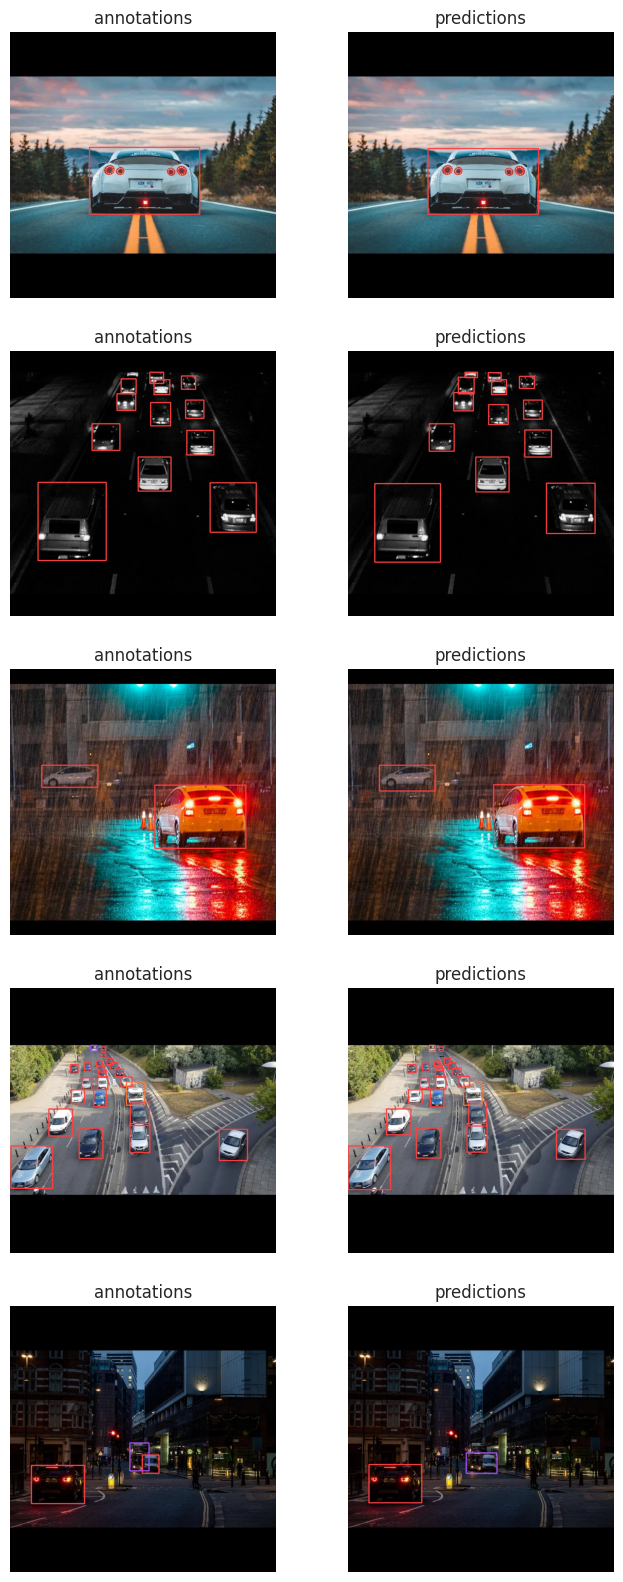
\includegraphics[width=0.6\linewidth]{tex/img/YNL2_Ann_Pred_2.png}
    \caption{Visualization of the performance of YOLO-NAS-L with bounding boxes and corresponding obstacle
classes predicted by the model.}
    \label{fig:L-annot-pred}
\end{figure}

\begin{figure}[H]
The Confusion Matrix illustrates the effectiveness of the overall YOLO-NAS-L in detecting obstacles across four distinct classes. Notably, the matrix reveals a notable variation in the true positive values. Specifically, the highest true positive rate, standing at 0.91 which is good, is achieved in detecting the 'motorbike' class. Conversely, the 'bus' class exhibits the lowest true positive rate, measured at 0.44 which is very poor.  
    \centering
    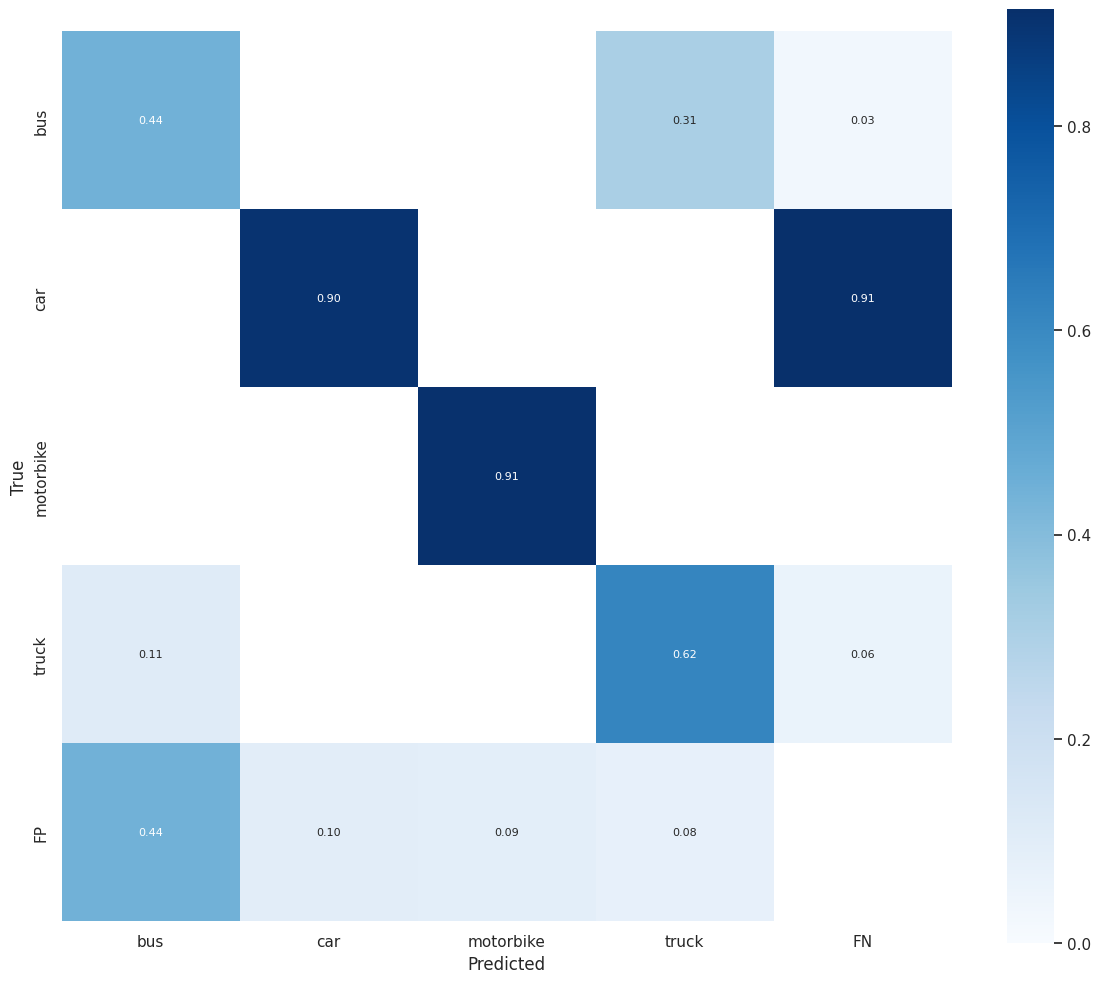
\includegraphics[width=\linewidth]{tex/img/YNL2_CM.png}
    \caption{YOLO-NAS-L Overall results }
    \label{fig:ConfusionMatrixY-N-L}
\end{figure}



\newpage
\subsection{Analysis of Performance for YOLO-NAS}
\begin{table}[htbp] 
\centering
\caption{Over-all results of the three models from the confusion matrix}
\label{tab:Comp}
\footnotesize
\begin{tabular}{|c|c|c|c|c|c|c|c|}%{ |c|c|c| }
\hline
\multicolumn{ 6}{|c|}{\textbf{YOLO-NAS-SMALL}}\\
\hline
\hline
\multirow{19}[1]{*}{True}
  & & Bus& Car& Motorbike& Truck \\
\hline
& Bus& \cellcolor[HTML]{00FFFF}{0.71}& & &  \\
\hline
& Car& & \cellcolor[HTML]{00FFFF}{0.93}& &  \\
\hline
& Motorbike& & & \cellcolor[HTML]{00FFFF}{1}&  \\
\hline
& Truck& & & & \cellcolor[HTML]{00FFFF}{0.55} \\ 
\hline
\hline
\multicolumn{ 6}{|c|}{\textbf{YOLO-NAS-MEDIUM}}\\
\hline
\hline
  & & Bus& Car& Motorbike& Truck \\
\hline
& Bus& \cellcolor[HTML]{00FFFF}{0.83}& & &  \\
\hline
& Car& & \cellcolor[HTML]{00FFFF}{0.87}& &  \\
\hline
& Motorbike& & & \cellcolor[HTML]{00FFFF}{0.91}&  \\
\hline
& Truck& & & & \cellcolor[HTML]{00FFFF}{0.56} \\ 
\hline
\hline
\multicolumn{ 6}{|c|}{\textbf{YOLO-NAS-LARGE}}\\
\hline
\hline
  & & Bus& Car& Motorbike& Truck \\
\hline
& Bus& \cellcolor[HTML]{00FFFF}{0.44}& & &  \\
\hline
& Car& & \cellcolor[HTML]{00FFFF}{0.90}& &  \\
\hline
& Motorbike& & & \cellcolor[HTML]{00FFFF}{0.91}&  \\
\hline
& Truck& & & & \cellcolor[HTML]{00FFFF}{0.62} \\ 
\hline
\hline
&  \multicolumn{ 5}{|c|}{\textbf{Predicted}}\\
\hline
\end{tabular}
\end{table}
The primary objective of table \ref{tab:Comp} is to provide a comprehensive analysis of the True Positive (TP) rate of three different models upon completion of their training. The table presents a comparative evaluation of the models' performance in detecting various classes, thus enabling researchers to identify the model that performs best. It is evident from the results that YOLO-NAS-M outperforms the other models in detecting all classes. Therefore, researchers can also fine-tune this model for future applications that require high accuracy in detecting various classes, similar to the training dataset mentioned in \ref{datset}.


%%%%%%%%%%%%%%%%%
\begin{table}[!htbp]
    \centering
    \caption{Analysis of Performance for YOLO-NAS}
    \label{tab:my_label}
    \footnotesize
    \begin{tabular}{|c|c|c|c|c|c|c|c|c|}
    \hline
     Models &  Loss\_cls&  Loss\_iou& Loss\_dfl & Loss &  Precision@0.5&  Recall@0.5&  mAP@0.5& F1@0.5\\
    \hline
    NAS-Small&  0.638&  0.122&  0.729&  1.308&  0.0717&  0.9327&  0.7812& 0.1323\\
    \hline
    NAS-Medium& 0.6198 &  0.1194&  0.7262&  1.2814& 0.0831 &  0.9308 & 0.8339 & 0.1513\\
    \hline
    NAS-Large& 0.6000 &  0.1154&  0.7355& 1.256 &  0.098&  0.9813&  0.8707& 0.1779\\
         \hline
    \end{tabular}
\end{table}

The performance metrics presented in Table \ref{tab:my_label} highlight interesting facets of the behavior of the different YOLO-NAS variants. First, the Recall scores for all models are exceptionally high, above 0.93 in all cases, which means that these models are very good at detecting the classes. This could be crucial in scenarios where the priority is to detect as many positive cases as possible, even at the risk of detecting some false classes.


Conversely, the precision scores present a contrasting narrative. The scores for all models are significantly lower, particularly in comparison to the high recall values. YOLO-NAS-L, the largest model, offers the best Precision at 0.098, YOLO-NAS-M at 0.0831, and YOLO-NASs at 0.0717. These low Precision scores suggest that while the models are good at capturing positive cases, they also have a high rate of false positives, this false positive is mostly coming from one class that is 'car' We can clearly see that in figure \ref{fig:ConfusionMatrixY-N-S}, \ref{fig:ConfusionMatrixY-N-M} \ref{fig:ConfusionMatrixY-N-L}

The F1-score, grows with the model size, reflecting that larger models achieve a better balance between these two measures.

The mAP@0.50 scores show that model size matters in delivering the best overall performance and that the larger models deliver the best overall performance.\\

In summary, while all the YOLO-NAS models exhibit
a strong ability to capture positive cases, they struggle with precision, indicating high false positives. Though marginally, the models’ complexity seems to positively influence precision and F1-score, suggesting potential benefits of
using larger models if computational resources and training time permit. However, the precision-recall trade-off must be carefully considered based on the specific requirements of the detection task.
